\chapter{ \toolName の外観と機能}\label{cha:Function}
本章では、本研究で試作したツール\toolName (Mix Visual Regression Test)の外観と機能について説明する。
\par
\toolName は、レイアウトの不具合の発見を支援する、視覚的回帰テスト支援ツールである。
WebページのURLを入力とし、Webページの画像とHTMLコードに基づいてレイアウトの不具合を含む可能性がある箇所を可視化した、
インターフェース(レイアウトの不具合確認画面ビュー)を出力する。【TODO: これを出力することでこういうことが分かるというのを考える。そうすればおのずと出力するものが分かるはず】
\par
\toolName の外観を、図\ref{fig: Appearance}に示す。
\begin{figure}[tp]
    \begin{center}
        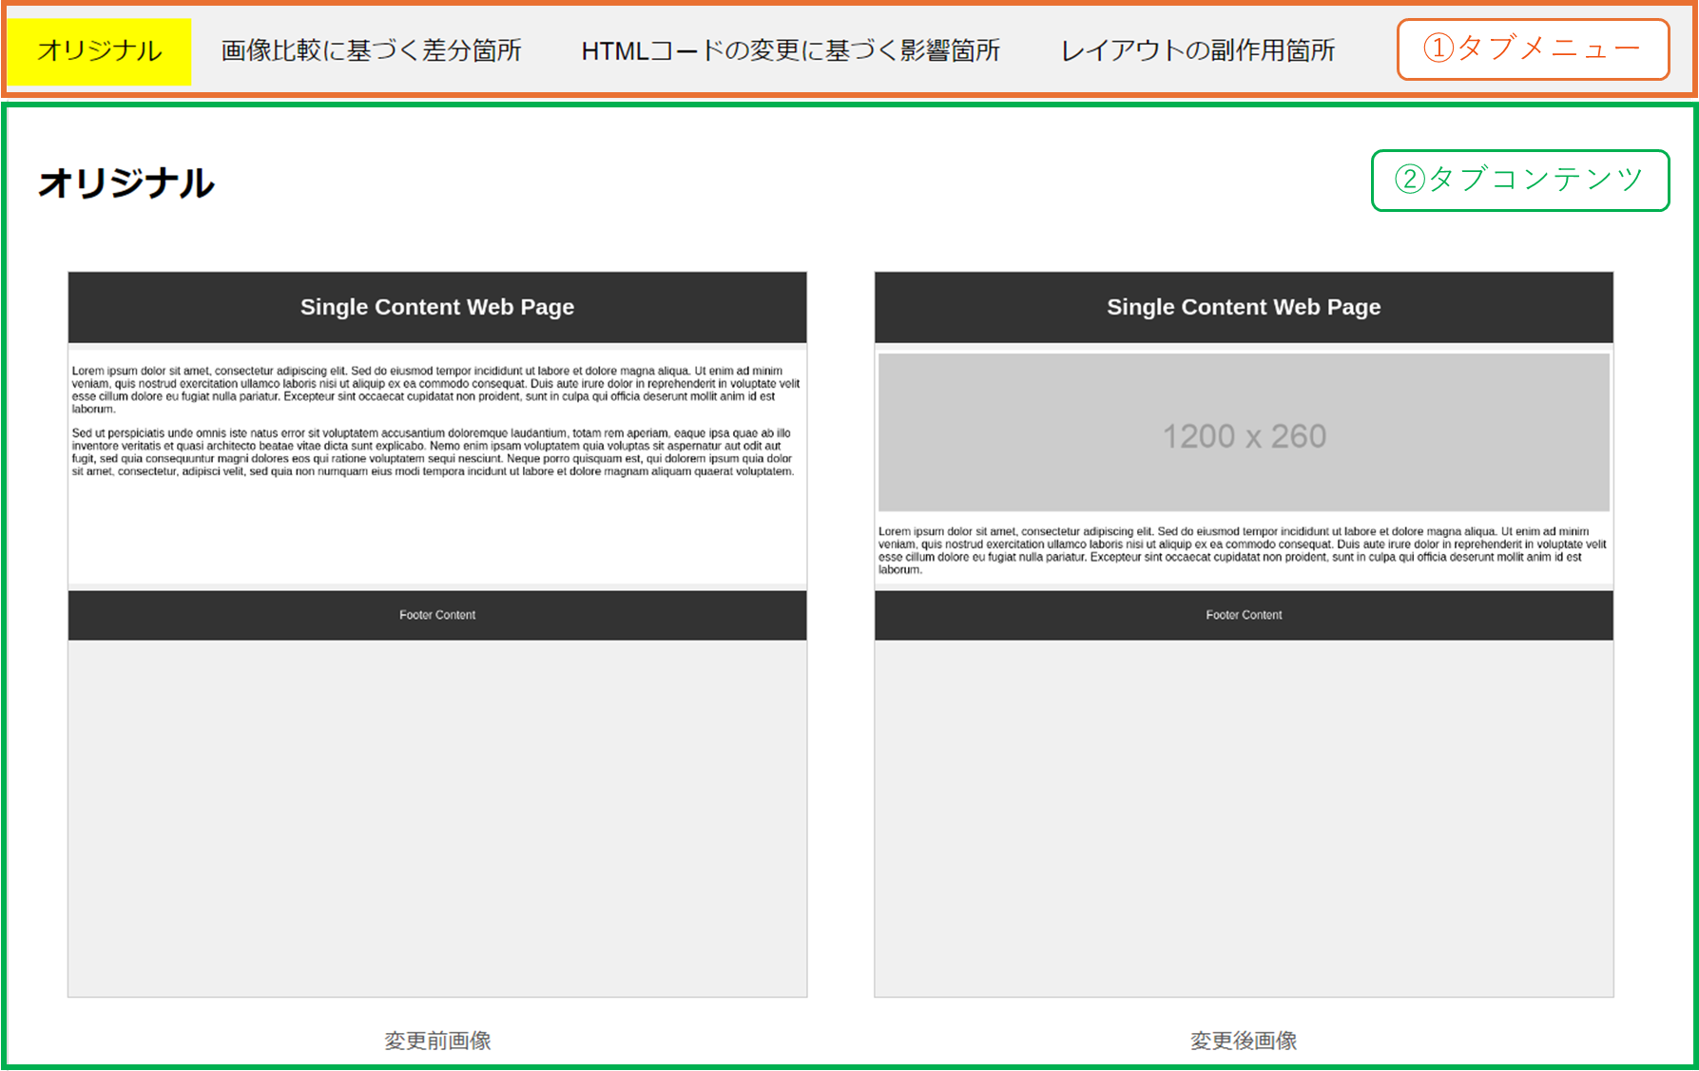
\includegraphics[width=1.0\columnwidth]{image/3_Outline_Appearance.png}
        \caption{\toolName の外観}
        \label{fig: Appearance}
    \end{center}
\end{figure}
% \toolName は、以下に示す4つのタブからなるタブメニューと各タブに対応した内容を表示するタブコンテンツからなる。
% なお、以下の数字は、図\ref{fig: Appearance}の数字と対応している。
% \begin{itemize}
%     \item タブメニュー
%     \item タブコンテンツ
% \end{itemize}
% \par
% また、タブメニューを構成する4つのタブは以下の通りである。
% \begin{itemize}
%     \item [①]オリジナル画像表示タブ
%     \item [②]画像比較に基づく差分箇所表示タブ
%     \item [③]HTMLコードの変更に基づく影響箇所表示タブ
%     \item [④]レイアウトの副作用箇所表示タブ
% \end{itemize}
% \par
% 以降、各タブの外観と機能について説明する。
% Webアプリケーションとして試作した\toolName は、以下に示す4つのタブからなるタブメニューと各タブに対応した内容を表示するタブコンテンツからなる。
% なお、以下の数字は、図\ref{fig: Appearance}の数字と対応している。
\toolName は、以下に示す4つのタブからなるタブメニューと各タブに対応した内容を表示するタブコンテンツからなる。
なお、以下の数字は、図\ref{fig: Appearance}の数字と対応している。
\begin{itemize}
    \item[①] タブメニュー
          \begin{itemize}
              \item オリジナル表示タブ
              \item 画像比較に基づく差分箇所表示タブ
              \item HTMLコードの変更に基づく影響箇所表示タブ
              \item レイアウトの副作用箇所表示タブ
          \end{itemize}
    \item[②] タブコンテンツ
\end{itemize}
\par
以降、各タブの外観と機能について説明する。



\section{オリジナル表示タブ}\label{subsec:original_tab}
オリジナル表示タブを押すと、Webページの変更前画像とWebページの変更後画像を表示する。
オリジナル表示タブを押した際の\toolName の画面例を、図\ref{fig: Appearance_original_tab}に示す。
なお、\toolName に一番最初にアクセスした時やリロードした時に、デフォルトでオリジナル表示タブを選択した状態になっている。
このタブでは、【TODO: ここでの目的を具体的に記述する】Webページの変更前後の画像を目視で確認できる。
\begin{figure}[tp]
    \begin{center}
        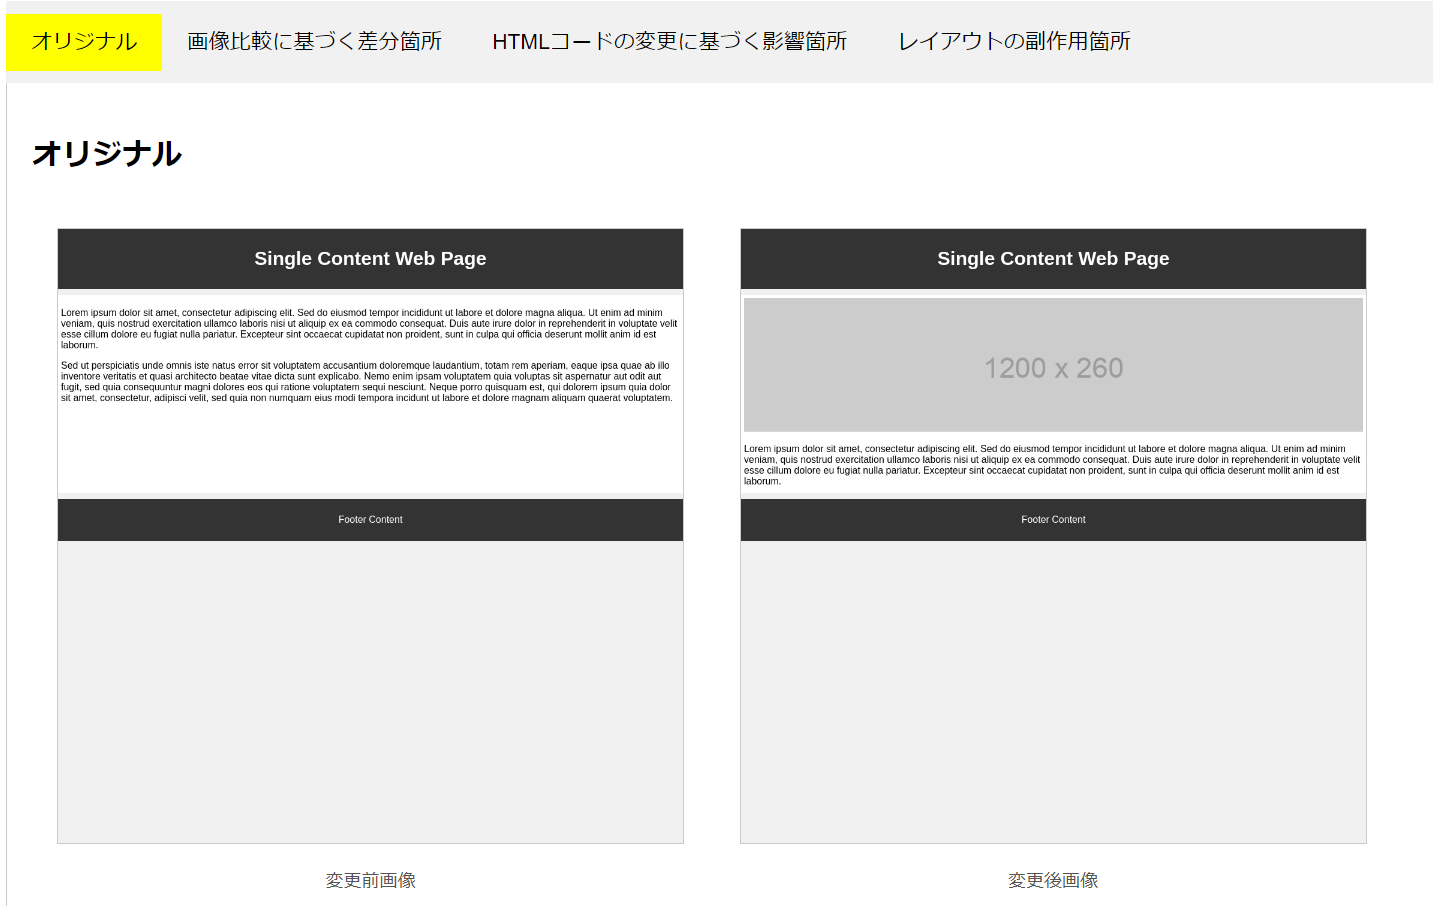
\includegraphics[width=1.0\columnwidth]{image/3_original_tab.png}
        \caption{オリジナル表示タブを押した際の\toolName の画面例}
        \label{fig: Appearance_original_tab}
    \end{center}
\end{figure}



\section{画像比較に基づく差分箇所表示タブ}\label{subsec:images_tab}
画像比較に基づく差分箇所表示タブを押すと、画像比較に基づく差分箇所を色付きの枠で囲んで強調表示した、Webページの変更前画像とWebページの変更後画像を表示する。
画像比較に基づく差分箇所表示タブを押した際の\toolName の画面例を、図\ref{fig: Appearance_images_tab}に示す。
ここでの差分箇所とは、変更前後のWebページを比較して、変更前のWebページで削除された箇所と変更後のWebページで追加された箇所を差分箇所と定義する。
削除された箇所は変更前画像上に赤枠で囲んで強調表示し、追加された箇所は変更後画像上に緑枠で囲んで強調表示する。
このタブでは、変更前後のWebページで画像比較によって差分が出た箇所を目視で確認できる。
\begin{figure}[tp]
    \begin{center}
        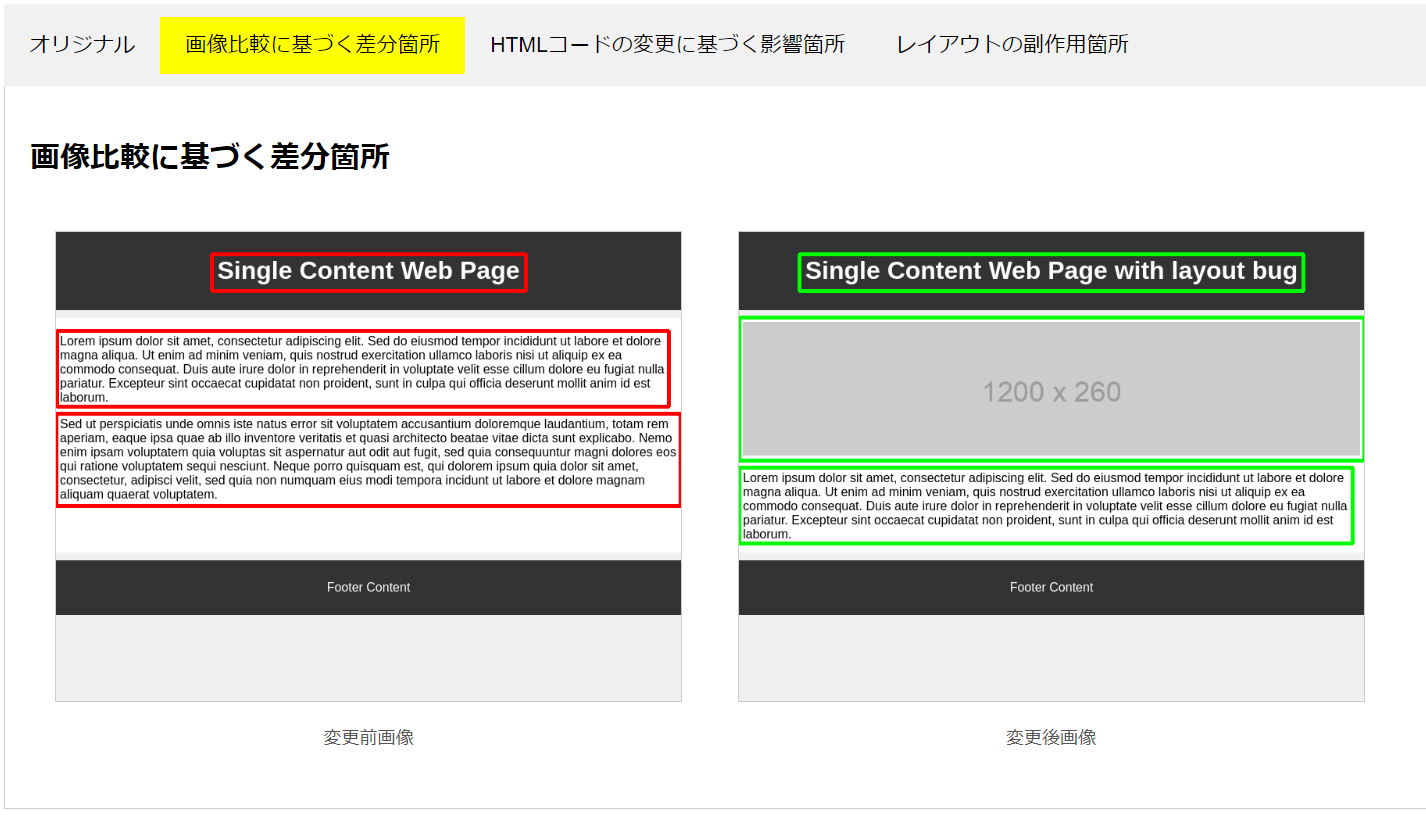
\includegraphics[width=1.0\columnwidth]{image/3_images_tab.png}
        \caption{画像比較に基づく差分箇所表示タブを押した際の\toolName の画面例}
        \label{fig: Appearance_images_tab}
    \end{center}
\end{figure}



\section{HTMLコードの変更に基づく影響箇所表示タブ}\label{subsec:html_tab}
HTMLの変更に基づく影響箇所表示タブを押すと、HTMLの変更に基づく影響箇所を色付きの枠で囲んで強調表示した、Webページの変更前画像とWebページの変更後画像を表示する。
HTMLの変更に基づく影響箇所表示タブを押した際の画面例を、図\ref{fig: Appearance_html_tab}に示す。
ここでの影響箇所とは、変更前後のWebページのHTMLコードを比較して、HTMLコードにおけるbody要素内の変更とstyle要素内の変更のどちらか、または両方の影響を受けた画面要素箇所と定義する。
変更前のWebページのHTMLでの影響箇所は変更前画像上に赤枠で囲んで強調表示し、変更後のWebページのHTMLでの影響箇所は変更後画像上に緑枠で囲んで強調表示する。
このタブでは、変更前後のWebページでHTMLコードの変更による影響を受けた画面要素を目視で確認できる。
% このタブでは、変更前後のWebページで開発者が意図したまたは意図しないHTMLコードの変更による影響箇所を目視で確認できる。
\begin{figure}[tp]
    \begin{center}
        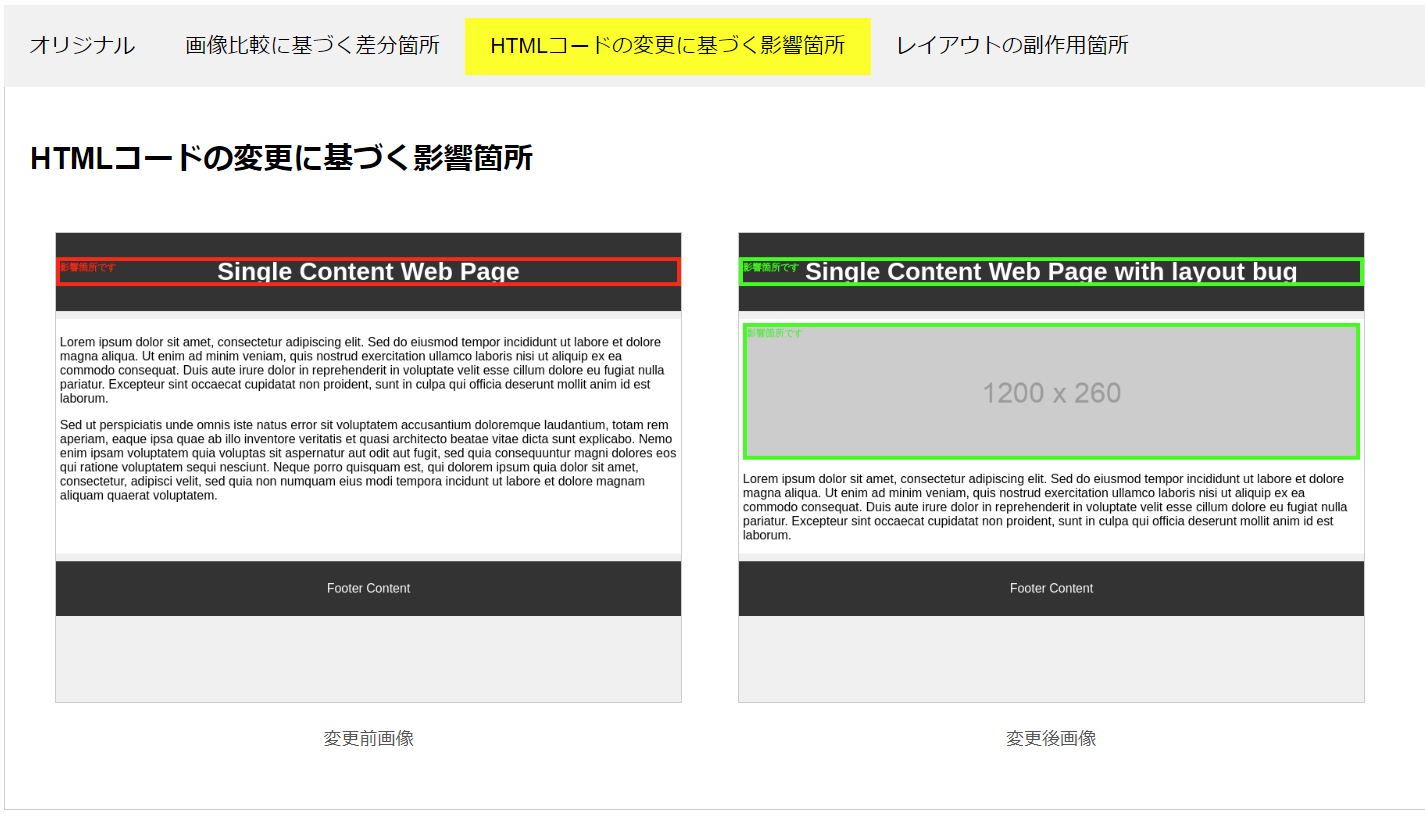
\includegraphics[width=1.0\columnwidth]{image/3_html_tab.png}
        \caption{HTMLコードの変更に基づく影響箇所表示タブを押した際の\toolName の画面例}
        \label{fig: Appearance_html_tab}
    \end{center}
\end{figure}



\section{レイアウトの副作用箇所表示タブ}\label{subsec:subeffect_tab}
レイアウトの副作用箇所表示タブを押すと、差分箇所と影響箇所に基づいて出力したレイアウトの副作用箇所を色付きの枠で強調表示した、Webページの変更前画像とWebページの変更後画像を表示する。
レイアウトの副作用箇所表示タブを押した際の画面例を、図\ref{fig: Appearance_subEffect_tab}に示す。
ここでのレイアウトの副作用箇所とは、変更前後のWebページでHTMLコードの変更による影響を受けた画面要素によって、HTMLコードを変更していない画面要素に見た目の変更があった箇所と定義する。
変更前のWebページでのレイアウトの副作用箇所は変更前画像上に赤枠で囲んで強調表示し、変更後のwebページでのレイアウトの副作用箇所は変更後画像上に緑枠で囲んで強調表示する。
このタブでは、変更前後のWebページでレイアウトの不具合を含む可能性のある箇所を目視で確認できる。
\begin{figure}[tp]
    \begin{center}
        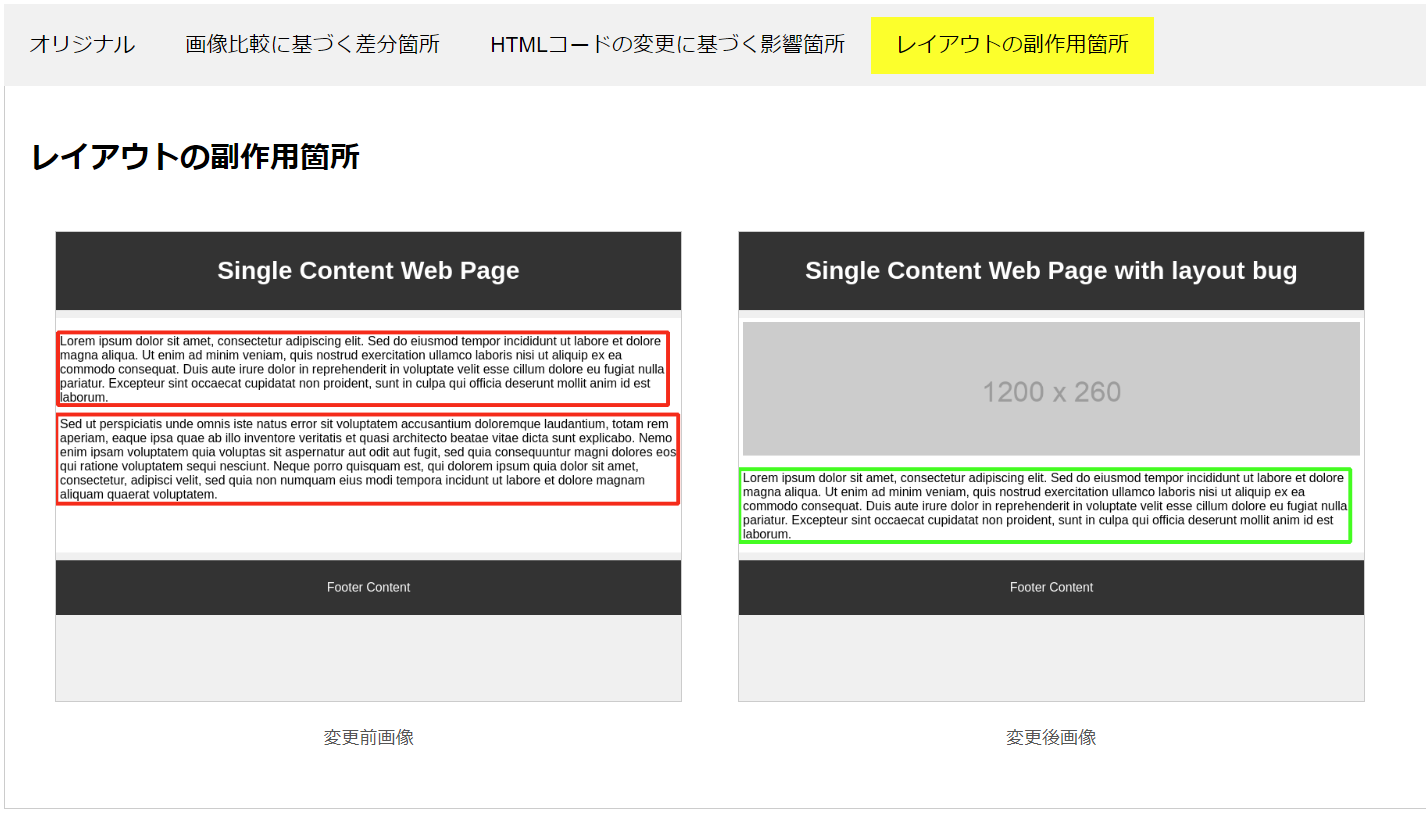
\includegraphics[width=1.0\columnwidth]{image/3_subEffect_tab.png}
        \caption{レイアウトの副作用箇所表示タブを押した際の\toolName の画面例}
        \label{fig: Appearance_subEffect_tab}
    \end{center}
\end{figure}

